% Options for packages loaded elsewhere
\PassOptionsToPackage{unicode}{hyperref}
\PassOptionsToPackage{hyphens}{url}
%
\documentclass[
  8pt,
  ignorenonframetext,
]{beamer}
\usepackage{pgfpages}
\setbeamertemplate{caption}[numbered]
\setbeamertemplate{caption label separator}{: }
\setbeamercolor{caption name}{fg=normal text.fg}
\beamertemplatenavigationsymbolsempty
% Prevent slide breaks in the middle of a paragraph
\widowpenalties 1 10000
\raggedbottom
\setbeamertemplate{part page}{
  \centering
  \begin{beamercolorbox}[sep=16pt,center]{part title}
    \usebeamerfont{part title}\insertpart\par
  \end{beamercolorbox}
}
\setbeamertemplate{section page}{
  \centering
  \begin{beamercolorbox}[sep=12pt,center]{part title}
    \usebeamerfont{section title}\insertsection\par
  \end{beamercolorbox}
}
\setbeamertemplate{subsection page}{
  \centering
  \begin{beamercolorbox}[sep=8pt,center]{part title}
    \usebeamerfont{subsection title}\insertsubsection\par
  \end{beamercolorbox}
}
\AtBeginPart{
  \frame{\partpage}
}
\AtBeginSection{
  \ifbibliography
  \else
    \frame{\sectionpage}
  \fi
}
\AtBeginSubsection{
  \frame{\subsectionpage}
}
\usepackage{amsmath,amssymb}
\usepackage{lmodern}
\usepackage{iftex}
\ifPDFTeX
  \usepackage[T1]{fontenc}
  \usepackage[utf8]{inputenc}
  \usepackage{textcomp} % provide euro and other symbols
\else % if luatex or xetex
  \usepackage{unicode-math}
  \defaultfontfeatures{Scale=MatchLowercase}
  \defaultfontfeatures[\rmfamily]{Ligatures=TeX,Scale=1}
\fi
% Use upquote if available, for straight quotes in verbatim environments
\IfFileExists{upquote.sty}{\usepackage{upquote}}{}
\IfFileExists{microtype.sty}{% use microtype if available
  \usepackage[]{microtype}
  \UseMicrotypeSet[protrusion]{basicmath} % disable protrusion for tt fonts
}{}
\makeatletter
\@ifundefined{KOMAClassName}{% if non-KOMA class
  \IfFileExists{parskip.sty}{%
    \usepackage{parskip}
  }{% else
    \setlength{\parindent}{0pt}
    \setlength{\parskip}{6pt plus 2pt minus 1pt}}
}{% if KOMA class
  \KOMAoptions{parskip=half}}
\makeatother
\usepackage{xcolor}
\newif\ifbibliography
\usepackage{color}
\usepackage{fancyvrb}
\newcommand{\VerbBar}{|}
\newcommand{\VERB}{\Verb[commandchars=\\\{\}]}
\DefineVerbatimEnvironment{Highlighting}{Verbatim}{commandchars=\\\{\}}
% Add ',fontsize=\small' for more characters per line
\usepackage{framed}
\definecolor{shadecolor}{RGB}{248,248,248}
\newenvironment{Shaded}{\begin{snugshade}}{\end{snugshade}}
\newcommand{\AlertTok}[1]{\textcolor[rgb]{0.94,0.16,0.16}{#1}}
\newcommand{\AnnotationTok}[1]{\textcolor[rgb]{0.56,0.35,0.01}{\textbf{\textit{#1}}}}
\newcommand{\AttributeTok}[1]{\textcolor[rgb]{0.77,0.63,0.00}{#1}}
\newcommand{\BaseNTok}[1]{\textcolor[rgb]{0.00,0.00,0.81}{#1}}
\newcommand{\BuiltInTok}[1]{#1}
\newcommand{\CharTok}[1]{\textcolor[rgb]{0.31,0.60,0.02}{#1}}
\newcommand{\CommentTok}[1]{\textcolor[rgb]{0.56,0.35,0.01}{\textit{#1}}}
\newcommand{\CommentVarTok}[1]{\textcolor[rgb]{0.56,0.35,0.01}{\textbf{\textit{#1}}}}
\newcommand{\ConstantTok}[1]{\textcolor[rgb]{0.00,0.00,0.00}{#1}}
\newcommand{\ControlFlowTok}[1]{\textcolor[rgb]{0.13,0.29,0.53}{\textbf{#1}}}
\newcommand{\DataTypeTok}[1]{\textcolor[rgb]{0.13,0.29,0.53}{#1}}
\newcommand{\DecValTok}[1]{\textcolor[rgb]{0.00,0.00,0.81}{#1}}
\newcommand{\DocumentationTok}[1]{\textcolor[rgb]{0.56,0.35,0.01}{\textbf{\textit{#1}}}}
\newcommand{\ErrorTok}[1]{\textcolor[rgb]{0.64,0.00,0.00}{\textbf{#1}}}
\newcommand{\ExtensionTok}[1]{#1}
\newcommand{\FloatTok}[1]{\textcolor[rgb]{0.00,0.00,0.81}{#1}}
\newcommand{\FunctionTok}[1]{\textcolor[rgb]{0.00,0.00,0.00}{#1}}
\newcommand{\ImportTok}[1]{#1}
\newcommand{\InformationTok}[1]{\textcolor[rgb]{0.56,0.35,0.01}{\textbf{\textit{#1}}}}
\newcommand{\KeywordTok}[1]{\textcolor[rgb]{0.13,0.29,0.53}{\textbf{#1}}}
\newcommand{\NormalTok}[1]{#1}
\newcommand{\OperatorTok}[1]{\textcolor[rgb]{0.81,0.36,0.00}{\textbf{#1}}}
\newcommand{\OtherTok}[1]{\textcolor[rgb]{0.56,0.35,0.01}{#1}}
\newcommand{\PreprocessorTok}[1]{\textcolor[rgb]{0.56,0.35,0.01}{\textit{#1}}}
\newcommand{\RegionMarkerTok}[1]{#1}
\newcommand{\SpecialCharTok}[1]{\textcolor[rgb]{0.00,0.00,0.00}{#1}}
\newcommand{\SpecialStringTok}[1]{\textcolor[rgb]{0.31,0.60,0.02}{#1}}
\newcommand{\StringTok}[1]{\textcolor[rgb]{0.31,0.60,0.02}{#1}}
\newcommand{\VariableTok}[1]{\textcolor[rgb]{0.00,0.00,0.00}{#1}}
\newcommand{\VerbatimStringTok}[1]{\textcolor[rgb]{0.31,0.60,0.02}{#1}}
\newcommand{\WarningTok}[1]{\textcolor[rgb]{0.56,0.35,0.01}{\textbf{\textit{#1}}}}
\setlength{\emergencystretch}{3em} % prevent overfull lines
\providecommand{\tightlist}{%
  \setlength{\itemsep}{0pt}\setlength{\parskip}{0pt}}
\setcounter{secnumdepth}{-\maxdimen} % remove section numbering
\newlength{\cslhangindent}
\setlength{\cslhangindent}{1.5em}
\newlength{\csllabelwidth}
\setlength{\csllabelwidth}{3em}
\newlength{\cslentryspacingunit} % times entry-spacing
\setlength{\cslentryspacingunit}{\parskip}
\newenvironment{CSLReferences}[2] % #1 hanging-ident, #2 entry spacing
 {% don't indent paragraphs
  \setlength{\parindent}{0pt}
  % turn on hanging indent if param 1 is 1
  \ifodd #1
  \let\oldpar\par
  \def\par{\hangindent=\cslhangindent\oldpar}
  \fi
  % set entry spacing
  \setlength{\parskip}{#2\cslentryspacingunit}
 }%
 {}
\usepackage{calc}
\newcommand{\CSLBlock}[1]{#1\hfill\break}
\newcommand{\CSLLeftMargin}[1]{\parbox[t]{\csllabelwidth}{#1}}
\newcommand{\CSLRightInline}[1]{\parbox[t]{\linewidth - \csllabelwidth}{#1}\break}
\newcommand{\CSLIndent}[1]{\hspace{\cslhangindent}#1}
% type setting
% ------------------------------------------------------------------------------
\usepackage[german]{babel}     

% fonts
% ------------------------------------------------------------------------------
\usefonttheme{professionalfonts}

% slide title and horizontal line
% ------------------------------------------------------------------------------
\setbeamertemplate{frametitle}{%
    \vskip-30pt \color{black}\large%
    \begin{minipage}[b][23pt]{120mm}%
    \flushleft\insertframetitle%
    \end{minipage}%
}

\setbeamertemplate{headline}										
{
\vskip10pt\hfill\hspace{3.5mm} 										 
\vskip15pt\color{black}\rule{\textwidth}{0.4pt} 					 
}

% slide number
% ---------------------------------------------------------------
\setbeamertemplate{navigation symbols}{}
\setbeamertemplate{footline}
{
\vskip5pt
\vskip2pt
\makebox[123mm]{\hspace{7.5mm}
\hfill Multivariate Datenanalyse $\vert$ 
\copyright $ $ 2023 Dirk Ostwald CC BY-SA 4.0 $\vert$ 
Folie \insertframenumber}
\vskip4pt
}

% block color scheme
% ------------------------------------------------------------------------------
% colors
\definecolor{white}{RGB}{255,255,255}
\definecolor{grey}{RGB}{235,235,235}
\definecolor{lightgrey}{RGB}{245,245,245}
\definecolor{LightBlue}{RGB}{220,220,255}
\definecolor{darkblue}{RGB}{51, 51, 153}

% definitions and theorems
\setbeamercolor{block title}{fg = black, bg = grey}
\setbeamercolor{block body}{fg = black, bg = lightgrey}

% general line spacing 
% ------------------------------------------------------------------------------
\linespread{1.3}

% local line spacing
% ------------------------------------------------------------------------------
\usepackage{setspace}

% colors
% -----------------------------------------------------------------------------
\usepackage{color}

% justified text
% ------------------------------------------------------------------------------
\usepackage{ragged2e}
\usepackage{etoolbox}
\apptocmd{\frame}{}{\justifying}{}

% bullet point lists
% -----------------------------------------------------------------------------
\setbeamertemplate{itemize item}[circle]
\setbeamertemplate{itemize subitem}[circle]
\setbeamertemplate{itemize subsubitem}[circle]
\setbeamercolor{itemize item}{fg = black}
\setbeamercolor{itemize subitem}{fg = black}
\setbeamercolor{itemize subsubitem}{fg = black}
\setbeamercolor{enumerate item}{fg = black}
\setbeamercolor{enumerate subitem}{fg = black}
\setbeamercolor{enumerate subsubitem}{fg = black}
\setbeamerfont{itemize/enumerate body}{}
\setbeamerfont{itemize/enumerate subbody}{size = \normalsize}
\setbeamerfont{itemize/enumerate subsubbody}{size = \normalsize}

% color links
% ------------------------------------------------------------------------------
\usepackage{hyperref}
\definecolor{urls}{RGB}{204,0,0}
\hypersetup{colorlinks, citecolor = darkblue, urlcolor = urls}


% additional math commands
% ------------------------------------------------------------------------------
\usepackage{bm}                               % bold math symbols
\usepackage{mathtools}                        % pmatrix* environment
\newcommand{\niton}{\not\owns}
\newcommand{\ups}{\upsilon}

% text highlighting
% ------------------------------------------------------------------------------
\usepackage{soul}
\makeatletter
\let\HL\hl
\renewcommand\hl{%
  \let\set@color\beamerorig@set@color
  \let\reset@color\beamerorig@reset@color
  \HL}
\makeatother

% equation highlighting
% -----------------------------------------------------------------------------
\newcommand{\highlight}[2][yellow]{\mathchoice%
  {\colorbox{#1}{$\displaystyle#2$}}%
  {\colorbox{#1}{$\textstyle#2$}}%
  {\colorbox{#1}{$\scriptstyle#2$}}%
  {\colorbox{#1}{$\scriptscriptstyle#2$}}}%

% additional mathematical operators
% ------------------------------------------------------------------------------
\DeclareMathOperator*{\argmax}{arg\,max}
\DeclareMathOperator*{\argmin}{arg\,min}

\ifLuaTeX
  \usepackage{selnolig}  % disable illegal ligatures
\fi
\IfFileExists{bookmark.sty}{\usepackage{bookmark}}{\usepackage{hyperref}}
\IfFileExists{xurl.sty}{\usepackage{xurl}}{} % add URL line breaks if available
\urlstyle{same} % disable monospaced font for URLs
\hypersetup{
  hidelinks,
  pdfcreator={LaTeX via pandoc}}

\author{}
\date{\vspace{-2.5em}}

\begin{document}

\begin{frame}[plain]{}
\protect\hypertarget{section}{}
\center

\begin{center}
\includegraphics[width=0.2\linewidth]{6_Abbildungen/mvda_6_otto} \end{center}

\vspace{2mm}

\Huge

Multivariate Datenanalyse \vspace{6mm}

\large

MSc Psychologie WiSe 2022/23

\vspace{6mm}
\large

Prof.~Dr.~Dirk Ostwald
\end{frame}

\begin{frame}[plain]{}
\protect\hypertarget{section-1}{}
\vfill
\center
\huge

\textcolor{black}{(6) Multivariate Normalverteilungen} \vfill
\end{frame}

\begin{frame}{}
\protect\hypertarget{section-2}{}
\setstretch{1.4}

\textcolor{darkblue}{Anwendungsfälle}

\small

Allgemeines Lineares Modell

\begin{itemize}
\tightlist
\item
  T-Tests, ANOVA, einfache und multiple Regression
\end{itemize}

Multivariates Allgemeines Lineares Modell

\begin{itemize}
\tightlist
\item
  T\(^2\)-Tests, MANOVA, einfache und multiple multivariate Regression
\end{itemize}

Hierarchische Modelle

\begin{itemize}
\tightlist
\item
  Linear Mixed Models, Bayesianische Regression, Diskriminanzanalyse
\end{itemize}

Lineare Normalverteilungsmodelle

\begin{itemize}
\tightlist
\item
  Probabilistische Hauptkomponentenanalyse, Faktorenanalyse
\end{itemize}

Kalman Filter, Gaussian Processes, Gaussian Random Fields, \ldots{}
\end{frame}

\begin{frame}{}
\protect\hypertarget{section-3}{}
\large
\setstretch{2.8}
\vfill

\textbf{Konstruktion und Definition}

Marginale Normalverteilungen

Gemeinsame Normalverteilungen

Bedingte Normalverteilungen

Selbstkontrollfragen \vfill
\end{frame}

\begin{frame}{Konstruktion und Definition}
\protect\hypertarget{konstruktion-und-definition}{}
\setstretch{1.3}
\footnotesize
\begin{definition}[Normalverteilte Zufallsvariable]
\justifying
$\xi$ sei eine Zufallsvariable mit Ergebnisraum $\mathbb{R}$ und WDF
\begin{equation}
p : \mathbb{R} \to \mathbb{R}_{>0}, x\mapsto p(x)
:= \frac{1}{\sqrt{2\pi \sigma^2}}\exp\left(-\frac{1}{2\sigma^2}(x - \mu)^2\right).
\end{equation}
Dann sagen wir, dass $\xi$ einer \textit{Normalverteilung (oder \textit{Gauß-Verteilung})
mit Parametern $\mu \in \mathbb{R}$ und $\sigma^2 > 0$} unterliegt und nennen $\xi$
eine \textit{normalverteilte Zufallsvariable}. Wir kürzen dies mit
$\xi \sim N(\mu,\sigma^2)$ ab. Die WDF einer normalverteilten
Zufallsvariable bezeichnen wir mit
\begin{equation}
N\left(x;\mu,\sigma^2\right) := \frac{1}{\sqrt{2\pi \sigma^2}}\exp\left(-\frac{1}{2\sigma^2}(x - \mu)^2\right).
\end{equation}
\end{definition}

Bemerkungen

\begin{itemize}
\tightlist
\item
  Es gelten \(\mathbb{E}(\xi) = \mu\) und
  \(\mathbb{V}(\xi) = \sigma^2\).
\item
  Der Parameter \(\mu\) entspricht dem Wert höchster
  Wahrscheinlichkeitsdichte.
\item
  Der Parameter \(\sigma^2\) spezifiziert die Breite der WDF.
\item
  \(\xi \sim N(0,1)\) heißt auch \emph{standardnormalverteilt}.
\end{itemize}
\end{frame}

\begin{frame}{Konstruktion und Definition}
\protect\hypertarget{konstruktion-und-definition-1}{}
\vspace{1mm}

\textcolor{darkblue}{Visualisierung univariater Normalverteilungsdichtefunktionen}
\vspace{1mm} \vspace{1cm}

\begin{center}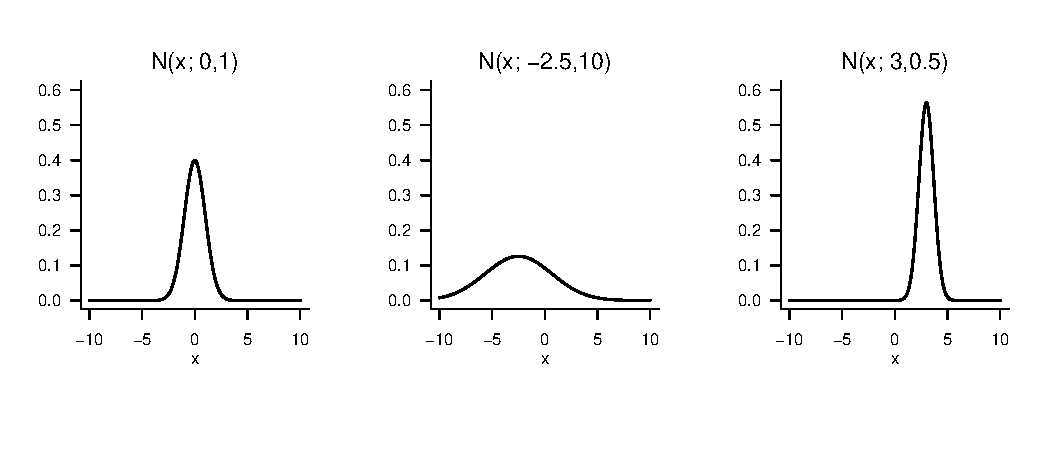
\includegraphics[width=1\linewidth]{6_Abbildungen/mvda_6_normalverteilung_wdf} \end{center}
\end{frame}

\begin{frame}{Konstruktion und Definition}
\protect\hypertarget{konstruktion-und-definition-2}{}
\footnotesize
\begin{theorem}[Konstruktion bivariater Normalverteilungen]
\justifying
\normalfont
$\zeta_1 \sim N(0,1)$ und $\zeta_2 \sim N(0,1)$ seien zwei unabhängige 
standardnormalverteilte  Zufallsvariablen. Weiterhin seien $\mu_1,\mu_2\in \mathbb{R}$,
$\sigma_1,\sigma_2>0$ und $\rho \in ]-1,1[$. Schließlich seien
\begin{align}
\begin{split}
\xi_1 & := \sigma_1\zeta_1 + \mu_1                                            \\
\xi_2 & := \sigma_2\left(\rho\zeta_1 + (1 -\rho^2)^{1/2}\zeta_2\right) + \mu_2. 
\end{split}
\end{align}
Dann hat die WDF des Zufallsvektors $\xi := (\xi_1,\xi_2)^T$, also der gemeinsamen 
Verteilung von $\xi_1$ und $\xi_2$, die Form
\begin{equation}
p : \mathbb{R}^2 \to \mathbb{R}_{>0},\, x \mapsto p(x)
:= (2\pi)^{-\frac{m}{2}}|\Sigma|^{-\frac{1}{2}}\exp\left(-\frac{1}{2}(x-\mu)^T \Sigma^{-1} (x-\mu)\right),
\end{equation}
wobei
\begin{equation}
m := 2,
\mu :=
\begin{pmatrix}
\mu_1 \\
\mu_2
\end{pmatrix}
\mbox{ und }
\Sigma :=
\begin{pmatrix}
\sigma_1^2           & \rho\sigma_1\sigma_2 \\
\rho\sigma_2\sigma_1 & \sigma_2^2           \\
\end{pmatrix}
\end{equation}

\end{theorem}

Bemerkungen

\begin{itemize}
\tightlist
\item
  Für einen Beweis siehe DeGroot and Schervish (2012), S. 338-339.
\item
  Man nennt die gemeinsame Verteilung von \(\xi_1\) und \(\xi_2\)
  \emph{bivariate Normalverteilung}.
\end{itemize}
\end{frame}

\begin{frame}[fragile]{Konstruktion und Definition}
\protect\hypertarget{konstruktion-und-definition-3}{}
\textcolor{darkblue}{Konstruktion bivariater Normalverteilungen}

\setstretch{.9}
\tiny

\begin{Shaded}
\begin{Highlighting}[]
\CommentTok{\# Parameterdefinitionen}
\NormalTok{mu\_1   }\OtherTok{=} \FloatTok{5.0}                                              \CommentTok{\# \textbackslash{}mu\_1}
\NormalTok{mu\_2   }\OtherTok{=} \FloatTok{4.0}                                              \CommentTok{\# \textbackslash{}mu\_2}
\NormalTok{sig\_1  }\OtherTok{=} \FloatTok{1.5}                                              \CommentTok{\# \textbackslash{}sigma\_1    }
\NormalTok{sig\_2  }\OtherTok{=} \FloatTok{1.0}                                              \CommentTok{\# \textbackslash{}sigma\_2}
\NormalTok{rho    }\OtherTok{=} \FloatTok{0.9}                                              \CommentTok{\# \textbackslash{}rho}

\CommentTok{\# Realisierungen der standardnormalverteilten ZVen}
\NormalTok{n      }\OtherTok{=} \DecValTok{100}                                              \CommentTok{\# Anzahl Realisierungen}
\NormalTok{zeta\_1 }\OtherTok{=} \FunctionTok{rnorm}\NormalTok{(n)                                         }\CommentTok{\# \textbackslash{}zeta\_1 \textbackslash{}sim N(0,1)  }
\NormalTok{zeta\_2 }\OtherTok{=} \FunctionTok{rnorm}\NormalTok{(n)                                         }\CommentTok{\# \textbackslash{}zeta\_1 \textbackslash{}sim N(0,1)}

\CommentTok{\# Evaluation von Realisierungen von \textbackslash{}xi\_1 und \textbackslash{}xi\_2}
\NormalTok{xi\_1   }\OtherTok{=}\NormalTok{ sig\_1}\SpecialCharTok{*}\NormalTok{zeta\_1 }\SpecialCharTok{+}\NormalTok{ mu\_1                              }\CommentTok{\# Realsierungen von zeta\_1  }
\NormalTok{xi\_2   }\OtherTok{=}\NormalTok{ sig\_2}\SpecialCharTok{*}\NormalTok{(rho}\SpecialCharTok{*}\NormalTok{zeta\_1 }\SpecialCharTok{+} \FunctionTok{sqrt}\NormalTok{(}\DecValTok{1}\SpecialCharTok{{-}}\NormalTok{rho}\SpecialCharTok{\^{}}\DecValTok{2}\NormalTok{)}\SpecialCharTok{*}\NormalTok{zeta\_2) }\SpecialCharTok{+}\NormalTok{ mu\_2 }\CommentTok{\# Realsierungen von zeta\_2  }


\CommentTok{\# Parameter der gemeinsamen Verteilung von \textbackslash{}xi\_1 und \textbackslash{}xi\_2}
\NormalTok{mu     }\OtherTok{=} \FunctionTok{matrix}\NormalTok{(}\FunctionTok{c}\NormalTok{(mu\_1,                                   }\CommentTok{\# \textbackslash{}mu \textbackslash{}in \textbackslash{}mathbb\{R\}\^{}2}
\NormalTok{                  mu\_2),  }
                 \AttributeTok{nrow =} \DecValTok{2}\NormalTok{, }\AttributeTok{byrow =} \ConstantTok{TRUE}\NormalTok{)}
\NormalTok{Sigma  }\OtherTok{=} \FunctionTok{matrix}\NormalTok{(}\FunctionTok{c}\NormalTok{(sig\_1}\SpecialCharTok{\^{}}\DecValTok{2}\NormalTok{        , rho}\SpecialCharTok{*}\NormalTok{sig\_1}\SpecialCharTok{*}\NormalTok{sig\_2,       }\CommentTok{\# \textbackslash{}Sigma \textbackslash{}in \textbackslash{}mathbb\{R\}\^{}\{2 x 2\}}
\NormalTok{                 rho}\SpecialCharTok{*}\NormalTok{sig\_1}\SpecialCharTok{*}\NormalTok{sig\_2, sig\_2}\SpecialCharTok{\^{}}\DecValTok{2}\NormalTok{),  }
                 \AttributeTok{nrow =} \DecValTok{2}\NormalTok{, }\AttributeTok{byrow =} \ConstantTok{TRUE}\NormalTok{)}
\FunctionTok{print}\NormalTok{(mu)}
\end{Highlighting}
\end{Shaded}

\begin{verbatim}
>      [,1]
> [1,]    5
> [2,]    4
\end{verbatim}

\begin{Shaded}
\begin{Highlighting}[]
\FunctionTok{print}\NormalTok{(Sigma)}
\end{Highlighting}
\end{Shaded}

\begin{verbatim}
>      [,1] [,2]
> [1,] 2.25 1.35
> [2,] 1.35 1.00
\end{verbatim}
\end{frame}

\begin{frame}{Konstruktion und Definition}
\protect\hypertarget{konstruktion-und-definition-4}{}
\vspace{2mm}

\textcolor{darkblue}{Konstruktion bivariater Normalverteilungen}

\center
\small

\textcolor{lightgray}{$\bullet$} Realisierungen von
\(\xi = (\xi_1,\xi_2)\), \(-\) Isokonturen von \(p\) \vspace{2mm}

\begin{center}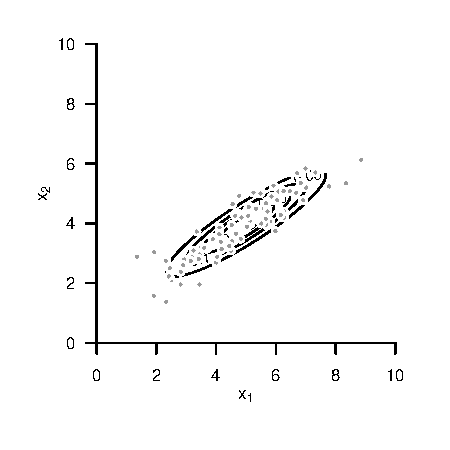
\includegraphics[width=0.55\linewidth]{6_Abbildungen/mvda_6_konstruktion} \end{center}
\end{frame}

\begin{frame}{Konstruktion und Definition}
\protect\hypertarget{konstruktion-und-definition-5}{}
\setstretch{1.3}
\footnotesize
\begin{definition}[Multivariate Normalverteilung]
\justifying
$\xi$ sei ein $m$-dimensionaler Zufallsvektor mit Ergebnisraum $\mathbb{R}^m$ und WDF
\begin{equation}
p : \mathbb{R}^m \to \mathbb{R}_{>0},\, x \mapsto p(x)
:= (2\pi)^{-\frac{m}{2}}|\Sigma|^{-\frac{1}{2}}\exp\left(-\frac{1}{2}(x-\mu)^T \Sigma^{-1} (x-\mu)\right).
\end{equation}
Dann sagen wird, dass $\xi$ einer \textit{multivariaten (oder $m$-dimensionalen)
Normalverteilung} mit \textit{Erwartungswertparameter} $\mu \in \mathbb{R}^m$ und
positive-definitem \textit{Kovarianzmatrixparameter} $\Sigma \in \mathbb{R}^{m \times m}$
unterliegt und nennen $\xi$ einen \textit{(multivariat) normalverteilten Zufallsvektor}.
Wir kürzen dies mit $\xi \sim N(\mu,\Sigma)$ ab. Die WDF eines multivariat
normalverteilten Zufallsvektors bezeichnen wir mit
\begin{equation}
N(x;\mu,\Sigma):= (2\pi)^{-\frac{m}{2}}|\Sigma|^{-\frac{1}{2}}\exp\left(-\frac{1}{2}(x-\mu)^T \Sigma^{-1} (x-\mu)\right).
\end{equation}
\end{definition}

Bemerkungen

\begin{itemize}
\tightlist
\item
  Es gelten \(\mathbb{E}(\xi) = \mu\) und \(\mathbb{C}(\xi) = \Sigma\).
\item
  Der Parameter \(\mu \in \mathbb{R}^m\) entspricht dem Wert höchster
  Wahrscheinlichkeitsdichte
\item
  Die Diagonalelemente von \(\Sigma\) spezifizieren die Breite der WDF
  bezüglich \(\xi_1,...,\xi_m\).
\item
  Das \(i,j\)te Element von \(\Sigma\) spezifiziert die Kovarianz on
  \(\xi_i\) und \(\xi_j\).
\item
  Der Term \((2\pi)^{-m/2}|\Sigma|^{-1/2}\) ist die
  Normalisierungskonstante für den Exponentialfunktionsterm.
\end{itemize}
\end{frame}

\begin{frame}[fragile]{Konstruktion und Definition}
\protect\hypertarget{konstruktion-und-definition-6}{}
\vspace{1mm}

\textcolor{darkblue}{Visualisierung bivariater Normalverteilungsdichtefunktionen}
\vspace{1mm} \tiny \setstretch{.9}

\begin{Shaded}
\begin{Highlighting}[]
\CommentTok{\# multivariate Normalverteilungstools}
\CommentTok{\# install.packages("mvtnorm")}
\FunctionTok{library}\NormalTok{(mvtnorm)}


\CommentTok{\# Ergebnisraumdefintion}
\NormalTok{x\_min  }\OtherTok{=} \DecValTok{0}                                           \CommentTok{\# x\_i Minimum}
\NormalTok{x\_max  }\OtherTok{=} \DecValTok{2}                                           \CommentTok{\# x\_i Maxim}
\NormalTok{x\_res  }\OtherTok{=} \FloatTok{1e3}                                         \CommentTok{\# x\_i Auflösung}
\NormalTok{x\_1    }\OtherTok{=} \FunctionTok{seq}\NormalTok{(x\_min, x\_max, }\AttributeTok{length.out =}\NormalTok{ x\_res)       }\CommentTok{\# x\_1 Raum}
\NormalTok{x\_2    }\OtherTok{=} \FunctionTok{seq}\NormalTok{(x\_min, x\_max, }\AttributeTok{length.out =}\NormalTok{ x\_res)       }\CommentTok{\# x\_2 Raum}
\NormalTok{X      }\OtherTok{=} \FunctionTok{expand.grid}\NormalTok{(x\_1,x\_2)                        }\CommentTok{\# X = (x\_1,x\_2)\^{}T Raum}

\CommentTok{\# Parameterdefinition}
\NormalTok{mu     }\OtherTok{=} \FunctionTok{c}\NormalTok{(}\DecValTok{1}\NormalTok{,}\DecValTok{1}\NormalTok{)                                      }\CommentTok{\# \textbackslash{}mu \textbackslash{}in \textbackslash{}mathbb\{R\}\^{}2}
\NormalTok{S      }\OtherTok{=} \FunctionTok{list}\NormalTok{(}\FunctionTok{matrix}\NormalTok{(}\FunctionTok{c}\NormalTok{(}\FloatTok{0.2}\NormalTok{,  }\FloatTok{0.15}\NormalTok{,  }\FloatTok{0.15}\NormalTok{, }\FloatTok{0.2}\NormalTok{), }\DecValTok{2}\NormalTok{),  }\CommentTok{\# \textbackslash{}Sigma in \textbackslash{}mathbb\{R\}\^{}\{2 \textbackslash{}times 2\}}
              \FunctionTok{matrix}\NormalTok{(}\FunctionTok{c}\NormalTok{(}\FloatTok{0.2}\NormalTok{,  }\FloatTok{0.00}\NormalTok{,  }\FloatTok{0.00}\NormalTok{, }\FloatTok{0.2}\NormalTok{), }\DecValTok{2}\NormalTok{),  }\CommentTok{\# \textbackslash{}Sigma in \textbackslash{}mathbb\{R\}\^{}\{2 \textbackslash{}times 2\}}
              \FunctionTok{matrix}\NormalTok{(}\FunctionTok{c}\NormalTok{(}\FloatTok{0.2}\NormalTok{, }\SpecialCharTok{{-}}\FloatTok{0.15}\NormalTok{, }\SpecialCharTok{{-}}\FloatTok{0.15}\NormalTok{, }\FloatTok{0.2}\NormalTok{), }\DecValTok{2}\NormalTok{))  }\CommentTok{\# \textbackslash{}Sigma in \textbackslash{}mathbb\{R\}\^{}\{2 \textbackslash{}times 2\}}

\CommentTok{\# Kovarianzparametervariantenschleife}
\ControlFlowTok{for}\NormalTok{ (Sigma }\ControlFlowTok{in}\NormalTok{ S)\{}

  \CommentTok{\# Wahrscheinlichkeitsdichtefunktionauswertung}
\NormalTok{  p      }\OtherTok{=} \FunctionTok{matrix}\NormalTok{(                                   }\CommentTok{\# Matrixkonversion des von}
                  \FunctionTok{dmvnorm}\NormalTok{(}\FunctionTok{as.matrix}\NormalTok{(X), mu, Sigma),  }\CommentTok{\# dmvnorm() ausgegebenen Vektors}
                  \AttributeTok{nrow =}\NormalTok{ x\_res)}

  \CommentTok{\# Visualisierung}
  \FunctionTok{contour}\NormalTok{(}
\NormalTok{  x\_1,}
\NormalTok{  x\_2,}
\NormalTok{  p,}
  \AttributeTok{xlim      =}  \FunctionTok{c}\NormalTok{(x\_min,x\_max),}
  \AttributeTok{ylim      =}  \FunctionTok{c}\NormalTok{(x\_min,x\_max),}
  \AttributeTok{nlevels   =} \DecValTok{5}\NormalTok{)\}}
\end{Highlighting}
\end{Shaded}
\end{frame}

\begin{frame}{Konstruktion und Definition}
\protect\hypertarget{konstruktion-und-definition-7}{}
\textcolor{darkblue}{Visualisierung bivariater Normalverteilungsdichtefunktionen}
\vspace{2mm}

\begin{center}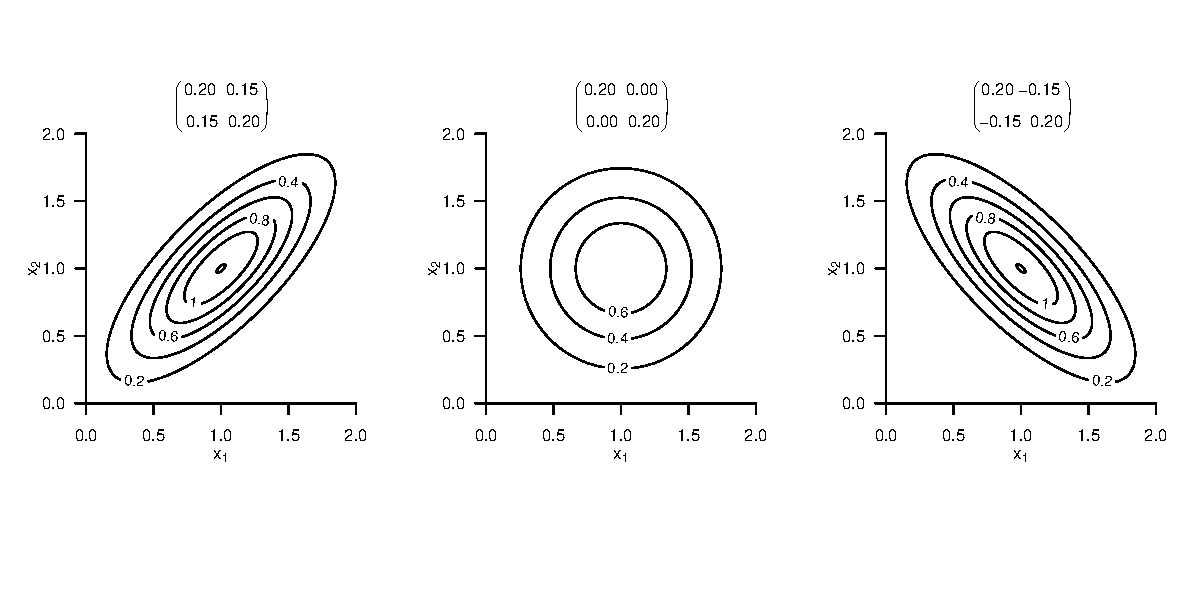
\includegraphics[width=1\linewidth]{6_Abbildungen/mvda_6_mvnwdf} \end{center}
\end{frame}

\begin{frame}[fragile]{Konstruktion und Definition}
\protect\hypertarget{konstruktion-und-definition-8}{}
\textcolor{darkblue}{Realisierung bivariater normalverteilter Zufallsvektoren}
\footnotesize \setstretch{1.1} \vspace{1mm}

\begin{Shaded}
\begin{Highlighting}[]
\CommentTok{\# R Paket für multivariate Normalverteilungen}
\FunctionTok{library}\NormalTok{(mvtnorm)}

\CommentTok{\# Parameterdefinition}
\NormalTok{mu     }\OtherTok{=} \FunctionTok{c}\NormalTok{(}\DecValTok{1}\NormalTok{,}\DecValTok{1}\NormalTok{)                                }\CommentTok{\# \textbackslash{}mu \textbackslash{}in \textbackslash{}mathbb\{R\}\^{}2}
\NormalTok{Sigma  }\OtherTok{=} \FunctionTok{matrix}\NormalTok{(}\FunctionTok{c}\NormalTok{(}\FloatTok{0.2}\NormalTok{,  }\FloatTok{0.15}\NormalTok{,  }\FloatTok{0.15}\NormalTok{, }\FloatTok{0.2}\NormalTok{), }\DecValTok{2}\NormalTok{)  }\CommentTok{\# \textbackslash{}Sigma in \textbackslash{}mathbb\{R\}\^{}\{2 \textbackslash{}times 2\}}

\CommentTok{\# Zufallsvektorrealisierungen}
\FunctionTok{rmvnorm}\NormalTok{(}\AttributeTok{n =} \DecValTok{10}\NormalTok{, mu, Sigma)}
\end{Highlighting}
\end{Shaded}

\begin{verbatim}
>        [,1]  [,2]
>  [1,] 1.552 0.975
>  [2,] 0.795 1.238
>  [3,] 0.172 0.242
>  [4,] 1.644 1.972
>  [5,] 0.449 0.221
>  [6,] 0.875 0.730
>  [7,] 0.639 0.682
>  [8,] 1.655 1.502
>  [9,] 0.887 0.381
> [10,] 1.405 1.255
\end{verbatim}
\end{frame}

\begin{frame}{Konstruktion und Definition}
\protect\hypertarget{konstruktion-und-definition-9}{}
\textcolor{darkblue}{Realisierung bivariater normalverteilter Zufallsvektoren}
\vspace{2mm}

\begin{center}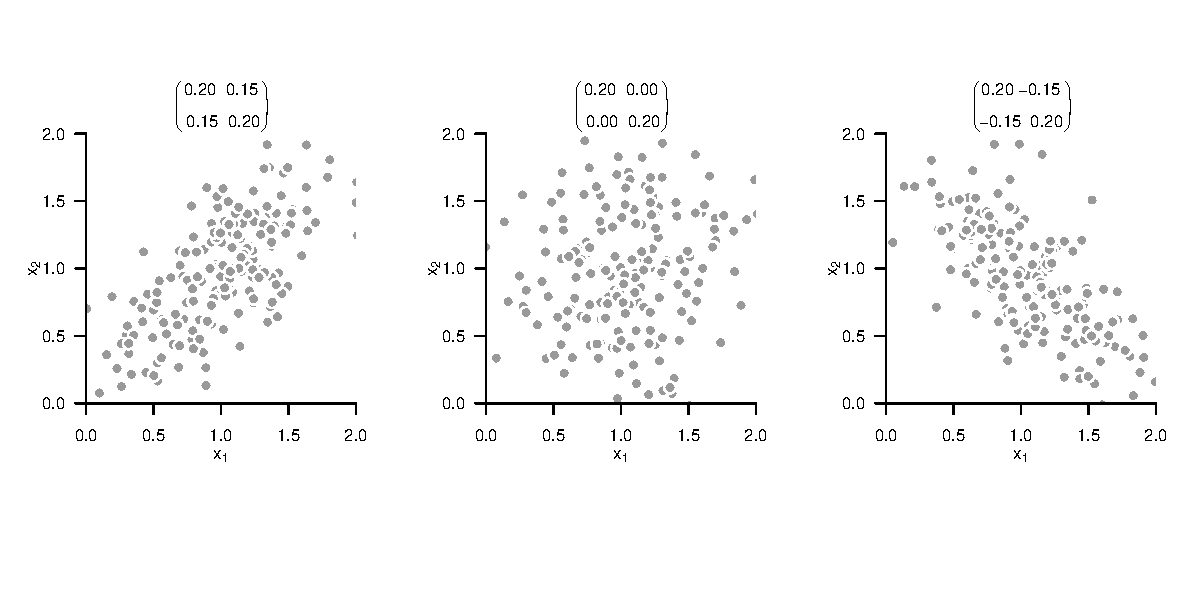
\includegraphics[width=1\linewidth]{6_Abbildungen/mvda_6_rmvnorm} \end{center}
\end{frame}

\begin{frame}{}
\protect\hypertarget{section-4}{}
\large
\setstretch{2.8}
\vfill

Konstruktion und Definition

\textbf{Marginale Normalverteilungen}

Gemeinsame Normalverteilungen

Bedingte Normalverteilungen

Selbstkontrollfragen \vfill
\end{frame}

\begin{frame}{Marginale Normalverteilungen}
\protect\hypertarget{marginale-normalverteilungen}{}
\footnotesize
\begin{theorem}[Marginale Normalverteilungen]
\justifying
\normalfont
Es sei $m := k + l$ und $\xi = (\xi_1,...,\xi_m)^T$ sei ein $m$-dimensionaler
normalverteilter Zufallsvektor mit Erwartungswertparameter
\begin{equation}
\mu =
\left(\begin{matrix}
\mu_\ups \\
\mu_\zeta
\end{matrix}\right) \in \mathbb{R}^m,
\end{equation}
mit $\mu_\ups \in \mathbb{R}^k$ and $\mu_\zeta \in \mathbb{R}^l$ und Kovarianzmatrixparameter
\begin{equation}
\Sigma =
\left(\begin{matrix}
\Sigma_{\ups\ups}   & \Sigma_{\ups\zeta} \\
\Sigma_{\zeta\ups}  & \Sigma_{\zeta\zeta}
\end{matrix}\right) \in \mathbb{R}^{m \times m},
\end{equation}
mit $\Sigma_{\ups\ups}   \in \mathbb{R}^{k \times k}$,
    $\Sigma_{\ups\zeta}  \in \mathbb{R}^{k \times l}$,
    $\Sigma_{\zeta\ups}  \in \mathbb{R}^{l \times k}$,
und $\Sigma_{\zeta\zeta} \in \mathbb{R}^{l \times l}$.
Dann sind $\ups := (\xi_1,...,\xi_k)^T$ und $\zeta := (\xi_{k+1}, ...,\xi_m)^T$
$k$- und $l$-dimensionale normalverteilte Zufallsvektoren, respektive, und es gilt
\begin{equation}
\ups \sim N(\mu_\ups,\Sigma_{\ups\ups}) \mbox{ and } \zeta \sim N(\mu_\zeta,\Sigma_{\xi\xi}),
\end{equation}
\end{theorem}

Bemerkungen

\begin{itemize}
\tightlist
\item
  Die Marginalverteilungen einer multivariaten Normalverteilung sind
  auch Normalverteilungen.
\item
  Die Parameter der Marginalverteilungen ergeben sich aus den Parametern
  der gemeinsamen Verteilung.
\item
  Für Beweise, siehe z.B. Mardia, Kent, and Bibby (1979), Kapitel 3 oder
  Anderson (2003), Kapitel.
\end{itemize}
\end{frame}

\begin{frame}{Marginale Normalverteilungen}
\protect\hypertarget{marginale-normalverteilungen-1}{}
\textcolor{darkblue}{Marginale Normalverteilungen} \small \center
\(m := 2, k = 1, l = 1, \mu := \begin{pmatrix} 1 \\ 2 \end{pmatrix}, \Sigma := \begin{pmatrix} 0.10 & 0.08 \\ 0.08 & 0.15 \end{pmatrix}\)

\vspace{-2mm}

\begin{center}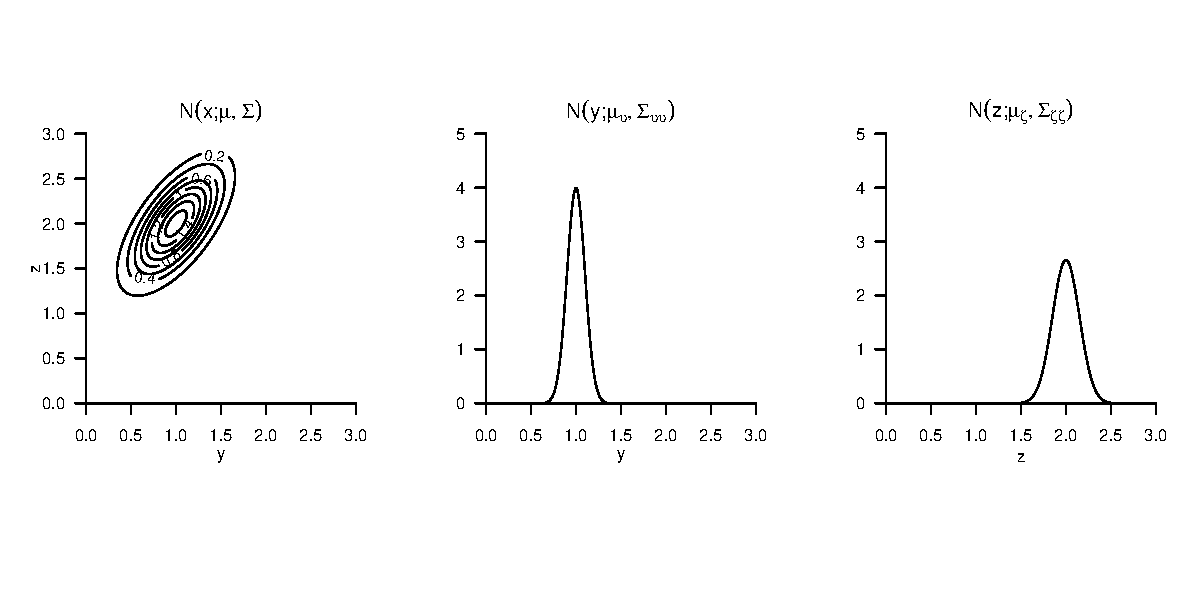
\includegraphics[width=1\linewidth]{6_Abbildungen/mvda_6_marginale_mvnorm} \end{center}
\end{frame}

\begin{frame}{}
\protect\hypertarget{section-5}{}
\large
\setstretch{2.8}
\vfill

Konstruktion und Definition

Marginale Normalverteilungen

\textbf{Gemeinsame Normalverteilungen}

Bedingte Normalverteilungen

Selbstkontrollfragen \vfill
\end{frame}

\begin{frame}{Gemeinsame Normalverteilungen}
\protect\hypertarget{gemeinsame-normalverteilungen}{}
\footnotesize
\begin{theorem}[Gemeinsame Normalverteilungen]
\justifying
\normalfont
$\xi$ sei ein $m$-dimensionaler normalverteilter Zufallsvektor mit WDF
\begin{equation}
p_\xi : \mathbb{R}^m \to \mathbb{R}_{>0},\,x\mapsto
p_\xi(x) := N(x;\mu_\xi,\Sigma_{\xi\xi}) \mbox{ mit }
\mu_\xi \in \mathbb{R}^m,
\Sigma_{\xi\xi} \in \mathbb{R}^{m\times m},
\end{equation}
$A\in\mathbb{R}^{n\times m}$ sei eine Matrix, $b\in\mathbb{R}^n$ sei ein Vektor
und $\ups$ sei ein $n$-dimensionaler bedingt normalverteilter Zufallsvektor mit
bedingter WDF
\begin{equation}
p_{\ups|\xi}(\cdot|x) : \mathbb{R}^n \to \mathbb{R}_{>0},\, y\mapsto
p_{\ups|\xi}(y|x) := N(y;A\xi+b,\Sigma_{\ups\ups}) \mbox{ mit }
\Sigma_{\ups\ups} \in \mathbb{R}^{n\times n}.
\end{equation}
Dann ist der $m+n$-dimensionale Zufallsvektor $(\xi,\ups)^T$ normalverteilt mit (gemeinsamer) WDF
\begin{equation}\label{eq:gauss_joint}
p_{\xi,\ups} : \mathbb{R}^{m+n} \to \mathbb{R}_{>0},\, \begin{pmatrix} x \\ y \end{pmatrix} \mapsto
p_{\xi,\ups}\left(\begin{pmatrix} x \\ y \end{pmatrix}\right) = N\left(\begin{pmatrix} x \\ y \end{pmatrix};
\mu_{\xi,\ups}, \Sigma_{\xi,\ups} \right),
\end{equation}
mit $\mu_{\xi,\ups} \in \mathbb{R}^{m+n}$ and $\Sigma_{\xi,\ups} \in \mathbb{R}^{m+n \times m+n}$ und insbesondere
\begin{equation}
\mu_{\xi,\ups} = \left( \begin{matrix} \mu_\xi \\ A\mu_\xi + b \end{matrix} \right)
\mbox{ und }
\Sigma_{\xi,\ups} = \left(\begin{matrix} \Sigma_{\xi\xi} & \Sigma_{\xi\xi}A^T \\ A\Sigma_{\xi\xi} & \Sigma_{\ups\ups} + A\Sigma_{\xi\xi}A^T \end{matrix} \right).
\end{equation}
\end{theorem}

Bemerkungen

\begin{itemize}
\tightlist
\item
  Eine marginale und eine bedingte multivariate Normalverteilung
  induzieren eine gemeinsame Normalverteilung.
\item
  Die Parameter der gemeinsamen Verteilungen ergeben sich als
  linear-affine Transformation der Parameter der induzierenden
  Verteilungen.
\end{itemize}
\end{frame}

\begin{frame}{Multivariate Normalverteilungen}
\protect\hypertarget{multivariate-normalverteilungen}{}
\textcolor{darkblue}{Gemeinsame Normalverteilungen} \small \vspace{2mm}
\center
\(m := 1, n := 1, \mu_\xi := 1, \Sigma_{\xi\xi} := 0.2, A := 1, b := 1, \Sigma_{\ups\ups} := 0.1\)
\vspace{-2mm}

\begin{center}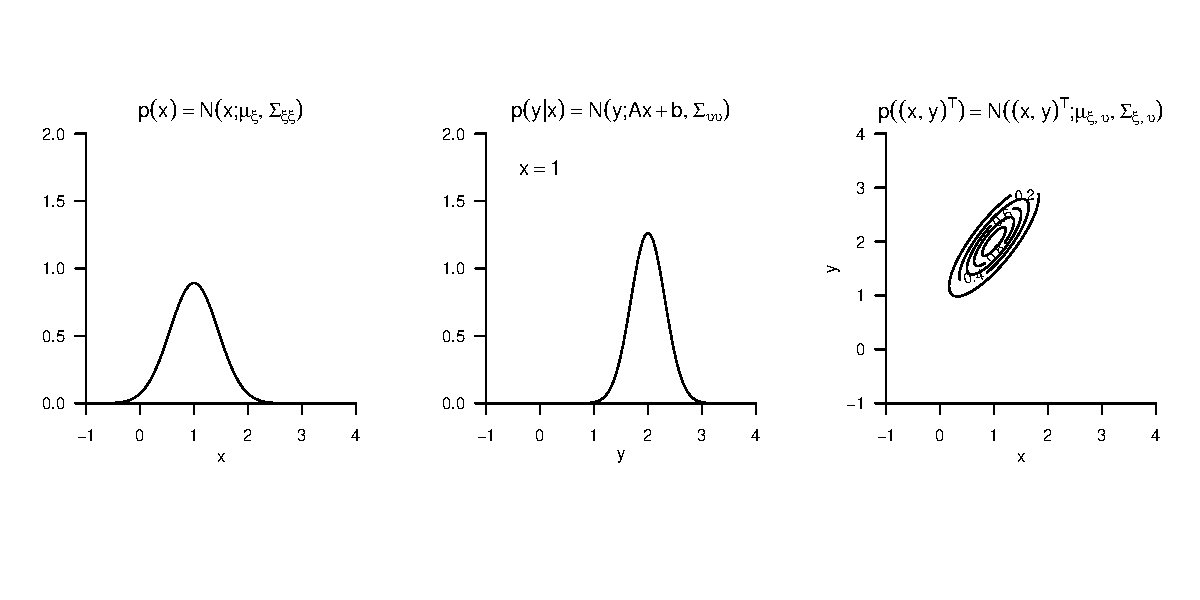
\includegraphics[width=1.05\linewidth]{6_Abbildungen/mvda_6_gemeinsame_mvnorm} \end{center}
\end{frame}

\begin{frame}{}
\protect\hypertarget{section-6}{}
\large
\setstretch{2.8}
\vfill

Konstruktion und Definition

Marginale Normalverteilungen

Gemeinsame Normalverteilungen

\textbf{Bedingte Normalverteilungen}

Selbstkontrollfragen \vfill
\end{frame}

\begin{frame}{Bedingte Normalverteilungen}
\protect\hypertarget{bedingte-normalverteilungen}{}
\footnotesize
\begin{theorem}[Bedingte Normalverteilungen]
\justifying
\normalfont
$(\xi,\ups)$ sei ein $m+n$-dimensionaler normalverteilter Zufallsvektor mit WDF
\begin{equation}
p_{\xi,\ups} : \mathbb{R}^{m + n} \to \mathbb{R}_{>0}, (x,y) \mapsto
p_{\xi,\ups}(x,y) := N\left((x,y); \mu_{\xi,\ups}, \Sigma_{\xi,\ups}\right),
\end{equation}
mit
\begin{equation}
\mu_{\xi,\ups} = \left(\begin{matrix} \mu_\xi \\ \mu_\ups \end{matrix} \right),
\Sigma_{\xi,\ups} = \left(\begin{matrix} \Sigma_{\xi\xi} & \Sigma_{\xi\ups} \\ \Sigma_{\ups\xi} & \Sigma_{\ups\ups} \end{matrix} \right),
\end{equation}
mit $x,\mu_\xi \in \mathbb{R}^m, y,\mu_\ups\in\mathbb{R}^n$ and  $\Sigma_{\xi\xi} \in \mathbb{R}^{m\times m}, \Sigma_{\xi\ups} \in \mathbb{R}^{m\times n}, \Sigma_{\ups\ups} \in \mathbb{R}^{n \times n}$. Dann ist die
bedingte Verteilung von $\xi$ gegeben $\ups$ eine $m$-dimensionale Normalverteilung
mit bedingter WDF
\begin{equation}
p_{\xi|\ups}(\cdot|y) : \mathbb{R}^m \to \mathbb{R}_{>0}, x \mapsto p_{\xi|\ups}(x|y) :=
N(x;\mu_{\xi|\ups},\Sigma_{\xi|\ups})
\end{equation}
mit
\begin{equation}\label{eq:gauss_cond_exp}
\mu_{\xi|\ups} = \mu_\xi  + \Sigma_{\xi\ups}\Sigma_{\ups\ups}^{-1}(\ups-\mu_\ups) \in \mathbb{R}^m
\end{equation}
und
\begin{equation}\label{eq:gauss_cond_var}
\Sigma_{\xi|\ups} = \Sigma_{\xi\xi}  - \Sigma_{\xi\ups}\Sigma_{\ups\ups}^{-1}\Sigma_{\ups\xi} \in \mathbb{R}^{m\times m}.
\end{equation}
\end{theorem}

Bemerkungen

\begin{itemize}
\tightlist
\item
  Die Parameter einer bedingten (multivariaten) Normalverteilung ergeben
  sich aus den Parametern einer gemeinsamen multivariaten
  Normalverteilung. Im Zusammenspiel mit den vorherigen Theoremen können
  die Parameter bedingter und marginale Normalverteilungen aus den
  Parametern der komplementären bedingten und marginalen
  Normalverteilungen bestimmt werden.
\end{itemize}
\end{frame}

\begin{frame}{Bedingte Normalverteilungen}
\protect\hypertarget{bedingte-normalverteilungen-1}{}
\textcolor{darkblue}{Bedingte Normalverteilungen} \small \center
\(m := 2, n := 1, \mu := \begin{pmatrix} 1 \\ 2 \end{pmatrix}, \Sigma := \begin{pmatrix} 0.12 & 0.09 \\ 0.09 & 0.12 \end{pmatrix}\)

\vspace{-2mm}

\begin{center}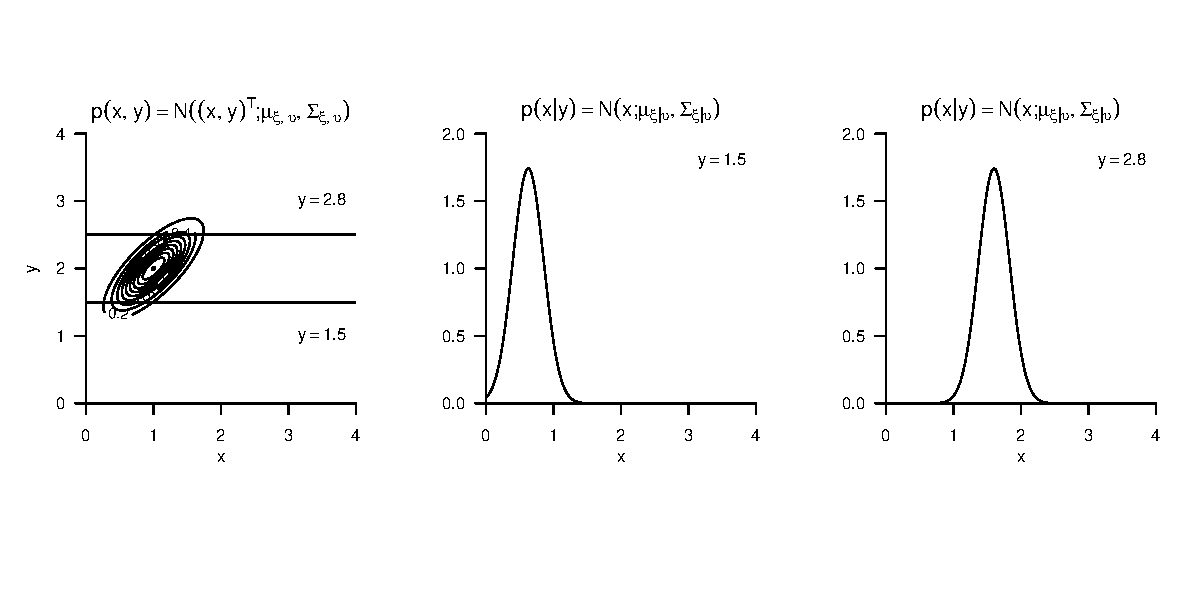
\includegraphics[width=1\linewidth]{6_Abbildungen/mvda_6_bedingte_mvnorm} \end{center}
\end{frame}

\begin{frame}{}
\protect\hypertarget{section-7}{}
\large
\setstretch{2.8}
\vfill

Konstruktion und Definition

Marginale Normalverteilungen

Gemeinsame Normalverteilungen

Bedingte Normalverteilungen

\textbf{Selbstkontrollfragen} \vfill
\end{frame}

\begin{frame}{Selbstkontrollfragen}
\protect\hypertarget{selbstkontrollfragen}{}
\setstretch{3}
\small
\begin{enumerate}
\item Definieren Sie die WDF einer univariaten normalverteilten Zufallsvariable.
\item Geben Sie das Theorem zur Konstruktion bivariater Normalverteilungen wieder.
\item Definieren Sie die WDF eines multivariaten normalverteilten Zufallsvektors.
\item Geben Sie das Theorem zu Marginalen Normalverteilungen wieder.
\item Geben Sie das Theorem zu Gemeinsamen Normalverteilungen wieder.
\item Geben Sie das Theorem zu Bedingten Normalverteilungen wieder.
\end{enumerate}
\end{frame}

\begin{frame}{Referenzen}
\protect\hypertarget{referenzen}{}
\footnotesize

\hypertarget{refs}{}
\begin{CSLReferences}{1}{0}
\leavevmode\vadjust pre{\hypertarget{ref-anderson_2003}{}}%
Anderson, T. W. 2003. \emph{An Introduction to Multivariate Statistical
Analysis}. 3rd ed. Wiley Series in Probability and Statistics. Hoboken,
N.J: Wiley-Interscience.

\leavevmode\vadjust pre{\hypertarget{ref-degroot_2012}{}}%
DeGroot, Morris H., and Mark J. Schervish. 2012. \emph{Probability and
Statistics}. 4th ed. Boston: Addison-Wesley.

\leavevmode\vadjust pre{\hypertarget{ref-mardia_1979}{}}%
Mardia, K. V., J. T. Kent, and J. M. Bibby. 1979. \emph{Multivariate
Analysis}. Probability and Mathematical Statistics. London ; New York:
Academic Press.

\end{CSLReferences}
\end{frame}

\end{document}
